\documentclass[12pt,
openright, 
oneside,
%twoside, %TCC: Se seu texto tem mais de 100 páginas, descomente esta linha e comente a anterior
a4paper,
brazil]{facom-ufu-abntex2}


######################### FUNDAMENTAÇÃO #############################33
\section{Referencial Teórico}
Para seguirmos uma linha de raciocínio linear, e melhorar entendimento da teoria
para compreender o projeto, será abordado inicialmente informações sobre o 
algoritmo Paxos, seu modo de operar e flexibilidade para resolução de problemas.

Em seguida, será explicado como é o funcionamento da linguagem P4, alguns exemplos
da sintaxe e como suas definições e um comparativo entre a versão utilizada neste 
projeto e a versão passada, $P4_{16}$ e $P4_{14}$, respectivamente. 
Também será explicado sobre o Mininet, seu funcionamento e qual o intuito na sua 
utilização no projeto. E para finalizar o referencial teórico, será explicado sobre o
Containernet, de que maneira funciona com o Mininet e como será utilizado.

###### P4 14 vs P4 16
\subsubsection{Comparação com a versão anterior}
Com a versão $P4_{16}$, foi realizado um trabalho, em que deixou uma lacuna de
incompatibilidade na semântica e sintaxe, quando comparada com a versão
$P4_{14}$, devido ao fato que diversos elementos da linguagem foram movidos
para arquivos externos, funcionando como bibliotecas, assim sendo necessário
importa os arquivos necessários para se utilizar dessas funcionalidades.

\begin{figure}[h]
    \caption{Mudança entre $P4_{14}$ para $P4_{16}$}
    \centering
    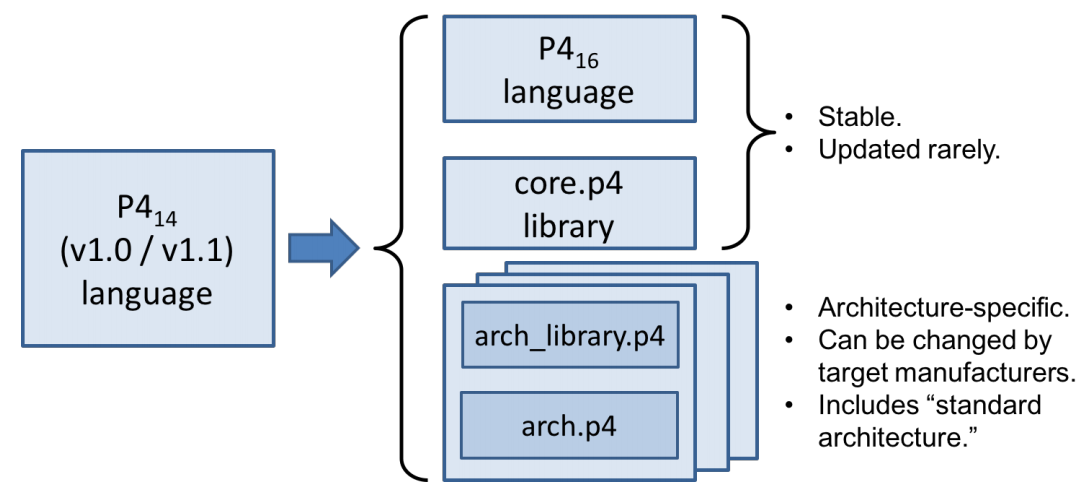
\includegraphics[width=\textwidth]{images/p414To16.png}
    \label{fig:language-comparison}
\end{figure}

Esse processo foi realizado para criar uma linguagem mais consistente, onde o núcleo da 
linguagem não sofrerá muitas alterações e se manterá compatível com futuras versões 
distribuídas, e caso não for possível manter a compatibilidade, viabilizar uma maneira 
fácil de realizar a migração entre versões da linguagem \citep{paxos16spec}. Com essas
alterações, é possível criar um distinção entre o que seria a arquitetura e o que se
é o alvo desenvolvido. Enquanto o alvo possui funções específicas e pode ser importado
por arquivos externos, oferecidos pelos próprios fornecedores a arquitetura é uma definição
abstrata do que se deseja utilizar

Um exemplo fornecido pelo documento de especificação da linguagem, demonstra a implementação
da arquitetura de um switch simples, de forma a demonstrar um exemplo  da linguagem,
utilizando a versão $P4_{16}$\citep{paxos16spec}. O exemplo a seguir define a arquitetura,
assim, o exemplo pode ser importado em outro projeto, que se utiliza da arquitetura para
seu funcionamento, o código é o seguinte:

\lstinputlisting[language=c++, caption={simple-switch-model.p4}]{code/p4-example/simple-switch.p4}

\subsection{Containernet}
Atualmente, diversas empresas utilizam o sistema de \textit{container} para disponibilizar seus 
serviços, empresas como PayPal e Visa \citep{dockerSite}. Com esse sistema a aplicação 
fica encapsulada em uma virtualização, onde tem tudo disponível para seu funcionamento, suas 
dependências, bibliotecas e configurações, assim separando a aplicação e suas dependências 
da infraestrutura \citep{dockerSite}. Assim, para realizar simulações o mais próximo possível
de ambientes utilizados por aplicações, será utilizado o Containernet.

Containernet se trata de um projeto derivado do Mininet, que possibilita a criação de
topologias de redes em que os \textit{hosts} são \textit{containers}. Esse ferramenta estende 
funcionalidades que não são possíveis de ser realizadas utilizando somente o Mininet
\citep{mininetDocs}. Utilizando o Containernet, é possível adicionar e remover 
\textit{containers} em tempo de execução, podendo simular uma infraestrutura da nuvem, onde os 
\textit{hosts} podem ser desligados, inseridos, e podem ter os seus recursos alterados
\citep{peuster2016medicine}.

\begin{figure}[h]
    \caption{Topologia utilizando Containernet}
    \centering
    
\includegraphics[width=\textwidth]{images/2d-2s-1c.png}
    \label{fig:containernet-topology-example}
\end{figure}

Para exemplificar como é realizada a construção de uma topologia utilizando Containernet, será
implementada uma topologia como da figura \ref{fig:containernet-topology-example}, utilizando
código em Python para tal, ficando da seguinte maneira:

\lstinputlisting[language=python,caption={containernet-topology.py}]{code/ninet-example/2dc-2sw-1c.py}

Desta forma, os 2 containers utilizam a imagem \texttt{ubuntu:trusty}, que pode ser encontrada
no Docker Hub \citep{dockerHub}, são adicionados 2 switches, que se comunicam com os
containers e entre si, a comunicação entre os switches possui um \textit{delay} de 100 ms.
Com a inicialização, a arquitetura definida será criada, em seguida o container \texttt{d1} envia um
\textit{ping} para o container \texttt{d2}. Para criar a topologia definida pelo arquivo 
\texttt{containernet-topology.py}, basta executar:

\begin{minted}{bash}
  $ sudo python containernet-topology.py
\end{minted}

Como notado pelo exemplo, a utilização do Containernet facilita a simulação do ambiente de 
produção de aplicações, onde será possível verificar o desempenho da implementação do Paxos
nos dispositivos de rede. Com a interface de utilização fácil, a criação de diferentes 
topologias para experimentos, diferentes opções para manejar os containers na rede,
faz com que o Containernet seja uma ferramente interessante para se utilizar no projeto.


\section{Cronograma}
O projeto foi realizado em dois semestres, cada semestre compreende 18 semanas, sendo assim,
um tempo total de desenvolvimento de 36 semanas ou aproximadamente 8 meses. A tabela 
\ref{tab:atividades} demonstra como foram realizadas as atividades no decorrer dos meses. 
% \todo{preferiria um cronograma semana a semana, dado que o prazo de execução é tão curto}

\begin{table}[!ht]
    \begin{tabular}{|p{8cm}|c|c|c|c|c|c|c|c|}
    \hline
    Atividades & 1 & 2 & 3 & 4 & 5 & 6 & 7 & 8 \\
    \hline
    \hline
     
    Revisão trabalhos correlatos & X & X & & & & & &  \\
    \hline 
    
    Revisão Paxos & & X & X & & & & & \\
    \hline
    
    Revisão P4 & & & X & X & & & & \\
    \hline
    
    Primeira fase do método & & & & X & & & & \\
    \hline
    
    Segunda fase do método & & & & & X & & & \\
    \hline
    
    Terceira fase do método & & & & & & X & & \\
    \hline
    
    Correção da monografia & & & & & & & X & \\
    \hline
    
    Monografia & & X & X & X & X & X & & \\
    \hline
    
    Defesa do trabalho de conclusão de curso & & & & & & & & X \\
    \hline
\end{tabular}
    \caption{Tabela de atividades}
    \label{tab:atividades}
\end{table}



\chapter{Conclusão}
Neste trabalho foi realizada a replicação e implementação de melhorias em um trabalho prévio \cite{dang2016paxos} utilizando
a linguagem de programação P4. Com a possibilidade de programação dos planos de dados em \textit{switches}, - foi demonstrado conceitualmente, 
utilizando simuladores - é possível mover a lógica de certas aplicações que são executadas em servidores para dispositivos de redes. O
exemplo utilizado para demonstração foi o algoritmo de consenso Paxos, que não é uma implementação trivial de ser realizada utilizando P4.
Algoritmos de consensos são centrais para construção de aplicações tolerante a falhas, uma mudança como trazer o algoritmo para dispositivos 
de rede, poderia melhorar na performance de \textit{data centers}. É possível observar que a possibilidade de implementação em dispositivos de redes 
viabiliza o desenvolvimento de novas pesquisas em um área ainda não tao explorada. Enquanto pesquisas em algoritmos de consensos já são bem maduras, 
pesquisas na implementação desses algoritmos para serem executados em dispositivos de redes, ainda não é uma área tão avançada \cite{dang2016paxos}. 